\SourcePage{GELFAND-P001228}{unlabelled}
\(\alpha_+,\alpha_-\), \(\alpha_+\alpha_-=-2\).
\Unclear{GELFAND-P001228}{equality-mark}{The small mark above the equals sign is illegible.}
\end{GelfandAdjacentEvidence}
\begin{GelfandAdjacentEvidence}{GELFAND-P001228}{2}

\begin{equation*}
\begin{aligned}
&\int_0^1
\prod_{\substack{i,j=1\\i<j}}^{n}(t_i-t_j)^{\alpha_+^2}
\prod_{\substack{n+1\le i,j\le n+m\\i<j}}(t_i-t_j)^{\alpha_-^2}
\left(\prod_{i=1}^{n+m}t_i\right)^\beta\\
&\qquad{}\cdot\prod_{\substack{1\le u\le n\\n+1\le v\le m+1}}(t_u-t_v)^{-2}\cdot\\
&\qquad{}\cdot\prod_{1\le i\le n}(z-t_i)^\gamma
\prod_{n+1\le i\le n+m}(z-t_i)^\delta\,dt_1\ldots dt_n.
\end{aligned}\tag{18}
\end{equation*}
\Unclear{GELFAND-P001228}{first-product-cancellation}{Notation is crossed out between \(i,j=1\) and \(i<j\) beneath the first product. Strokes resembling \(i\) and \(j\) are visible. The sign between them is illegible.}
\end{GelfandAdjacentEvidence}
\begin{GelfandAdjacentEvidence}{GELFAND-P001228}{3}

\Unclear{GELFAND-P001228}{mixed-product-cancellation}{An illegible mark is crossed out beneath the two constraints on the mixed product.}
\end{GelfandAdjacentEvidence}
\begin{GelfandAdjacentEvidence}{GELFAND-P001228}{4}

\EvidenceBlock{GELFAND-P001228}{integral-index-mismatch}{The upper bound for \(v\) is written \(m+1\). The final differential is written \(dt_n\).}{Manuscript notation.}
\end{GelfandAdjacentEvidence}
\begin{GelfandAdjacentEvidence}{GELFAND-P001228}{5}


In this form the 2-point correlation fn. of the theory (conformal field theory) is represented.

[crossed out] This gives a [schetnoe?] number of correlation fns.
\Unclear{GELFAND-P001228}{prose-cancellation}{The crossed-out word before “This gives” may read «Если» (Esli).}
\end{GelfandAdjacentEvidence}
\begin{GelfandAdjacentEvidence}{GELFAND-P001228}{6}

\Unclear{GELFAND-P001228}{count-word}{The word before “number” tentatively reads «счетное» (schetnoe). Its ending «етное» is legible and its opening strokes are unclear.}
\end{GelfandAdjacentEvidence}
\begin{GelfandAdjacentEvidence}{GELFAND-P001228}{7}


The real fns. are their analytic continuation to complex \(n\) and \(m\).

\uwave{It is called 4-point} (although it depends only on \(z\)).

[A short stroke leads down from \(z\)] [crossed out] cross-ratio of 4 points on \(CP^1\).
\Unclear{GELFAND-P001228}{marginal-cancellation}{The crossed-out word before “cross-ratio” may read «она» (ona).}
\end{GelfandAdjacentEvidence}
\begin{GelfandAdjacentEvidence}{GELFAND-P001228}{8}

\EvidenceBlock{GELFAND-P001228}{correlation-order}{The upper passage reads “2-point”. The lower passage reads “4-point”, with a raised and underlined х after the numeral.}{Manuscript notation.}
\end{GelfandAdjacentEvidence}



\Needspace{7\baselineskip}
\begin{GelfandAdjacentEvidence}{GELFAND-P001229}{1}
\SourcePage{GELFAND-P001229}{unlabelled}
\underline{\(11/\overline{\underline{\mathrm{XI}}}-85\)  }\qquad
\underline{Gelfand Sem.}

\underline{\underline{Vershik A. M.}}\qquad \underline{Topology of configuration space[?].}
\Unclear{GELFAND-P001229}{title-word}{The legible stem is «пространств» (prostranstv). The inked-over final sign is tentatively «а» (a). A separate dot is visible to its right.}
\end{GelfandAdjacentEvidence}
\begin{GelfandAdjacentEvidence}{GELFAND-P001229}{2}


\(1^{\circ}.\)
\SourceFigure{GELFAND-P001229}{grassmann-membership}{%
\par\smallskip
{\color{black}\begingroup\color{black}\GelfandFitDiagram{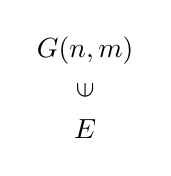
\begin{tikzpicture}
\node at (0,0) {\(G(n,m)\)};
\node[rotate=90] at (0,-.5) {\(\in\)};
\node at (0,-1) {\(E\)};
\end{tikzpicture}}\endgroup}\par\smallskip}
\end{GelfandAdjacentEvidence}
\begin{GelfandAdjacentEvidence}{GELFAND-P001229}{3}

\(e_1,\ldots,e_n\) --- basis in \(\mathbb R^n\)
\begin{equation*}
\tau_E=(Pe_1,\ldots,Pe_n)
\end{equation*}
What is the top. stratum in \(G(n,m)\), where \(\tau_E\) has a given combinat. type?

\(2^{\circ}.\) Combinat. theory of convex polyhedra in \(\mathbb R^n\).

2 polyhedra \(V_1,V_2\) with ordered (numbered) vertices (\(n\) of them)
[crossed out] have the same combinat. type if their faces correspond to each other.
\Incomplete{GELFAND-P001229}{cancelled-type}{The crossed-out passage after “\(n\) of them” is undeciphered.}
\end{GelfandAdjacentEvidence}
\begin{GelfandAdjacentEvidence}{GELFAND-P001229}{4}


Grassmannization of the problem.

In \(\mathbb R^n\) consider a subspace (\(m\)-dimensional) \(E\)
\begin{equation*}
S=\omega(e_1,\ldots,e_n)\quad\text{--- simplex}
\end{equation*}
\EvidenceBlock{GELFAND-P001229}{simplex-symbol}{The sign after the equals sign is \(\omega\).}{Manuscript notation.}
\end{GelfandAdjacentEvidence}
\begin{GelfandAdjacentEvidence}{GELFAND-P001229}{5}

The projection of \(S\) onto \(E\) --- polyhedron (convex)

\underline{Ex.:} obtain combinatorially any polyhedron of dim. \(m\) with \(n\) vertices

On \(G(n,m)\) consider the partition into subsets where the polyhedra carried by the subspace are combinatorially equivalent.
\EvidenceBlock{GELFAND-P001229}{subspace-abbreviation}{The abbreviation after “carried” is «подпр-вом» (podpr-vom, “by the subspace”).}{Manuscript notation.}
\end{GelfandAdjacentEvidence}
\begin{GelfandAdjacentEvidence}{GELFAND-P001229}{6}


What is the topology of these pieces?

\(3^{\circ}.\)
\SourceFigure{GELFAND-P001229}{matrix-hatching}{%
\par\smallskip
{\color{black}\(\begin{array}{c}
\left(\begin{array}{@{}ccc@{}}
x_{11}&\cdots&x_{1n}\\
x_{21}&\cdots&x_{2n}\\
x_{31}&\cdots&x_{3n}\\
\hline
\multicolumn{3}{c}{\text{\tikz[x=.65cm,y=.40cm]{
\draw (0,.02)--(.37,.26)--(.24,.04)--(.74,.24)--(.61,.02)--(1.13,.24)--(1.00,.03)--(1.54,.22)--(1.39,.01)--(1.89,.23);}}}
\end{array}\right)
\qquad
\begin{pmatrix}
x'_{11}&\cdots&x'_{1n}\\
x'_{21}&\cdots&x'_{2n}\\
x'_{31}&\cdots&x'_{3n}
\end{pmatrix}\\[3pt]
\text{--- 2 matrices }3\times n
\end{array}\)}\par\smallskip
A rule and looping hatching lie under the third row of the first matrix. The purpose of the hatching is unclear. The second matrix has neither mark.}
\end{GelfandAdjacentEvidence}


Let all minors be \(\ne0\) and have the same signs for \(x\) and \(x'\).

Does there exist a homotopy \(x(t)\) of matrices with \(x(0)=x\), \(x(1)=x'\)


\Needspace{7\baselineskip}
\begin{GelfandAdjacentEvidence}{GELFAND-P001230}{1}
\SourcePage{GELFAND-P001230}{15}
in the same class?
\begin{gather*}
n\le7\ \Rightarrow\ \text{possible}\\
n=19\ \Rightarrow\ \text{impossible!}\qquad\text{(N. E. Mnëv)}
\end{gather*}
Configurations also make sense in \(\mathbb RP^n\) and one needs to supplement.
\EvidenceBlock{GELFAND-P001230}{configuration-end}{The final word reads «дополнять» (dopolnyat', “to supplement”).}{Manuscript notation.}
\end{GelfandAdjacentEvidence}
\begin{GelfandAdjacentEvidence}{GELFAND-P001230}{2}


One needs to [probe?] the consequences (by projection) and there is a bound on how many one needs to take to have enough.
\Unclear{GELFAND-P001230}{consequences-verb}{The joined strokes tentatively read «пощупать» (poshchupat', “to probe”). The following word “consequences” is legible.}
\end{GelfandAdjacentEvidence}
\begin{GelfandAdjacentEvidence}{GELFAND-P001230}{3}

\EvidenceBlock{GELFAND-P001230}{consequences-parenthesis}{The parenthesis reads «проектированием» (proektirovaniem, “by projection”). It is followed by “and there is a bound.”}{Manuscript notation.}
\end{GelfandAdjacentEvidence}
\begin{GelfandAdjacentEvidence}{GELFAND-P001230}{4}


The topology can be that of any algebraic var.!

(This is over \(\mathbb R\))

over \(C\) the analogue is computing \(\pi_1\).

It is interesting what the convex analogue is over \(C\).

\underline{Steinitz's thm.}: characterization of the 1-dim. skeleton of a convex polyhedron

(see any textbook of convex geom.) (in \(\mathbb R^3\))

\underline{Corollary}: the space of polyhedra of a given combinat. type in \(\mathbb R^3\) is contractible.

\underline{But}: in \(\mathbb R^4\) there already exist even simplicial polyhedra
with more or less any [crossed out] topology of combinat. type.
\Incomplete{GELFAND-P001230}{topology-cancel}{The crossed-out word between “any” and “topology” is undeciphered.}
\end{GelfandAdjacentEvidence}
\begin{GelfandAdjacentEvidence}{GELFAND-P001230}{5}


\uwave{Problem}: we want to construct a field of polyhedra on a manifold! (in each tangent sp.).
There was [crossed out] a classific. problem for this one.
\Incomplete{GELFAND-P001230}{classification-cancel}{The crossed-out passage after “There was” is undeciphered.}
\end{GelfandAdjacentEvidence}
\begin{GelfandAdjacentEvidence}{GELFAND-P001230}{6}


\uwave{Matroids} [m.?] Given a lattice. It is called a \uwave{geometric lattice},
if it is
\begin{enumerate}
\item[1)] Semimodular
\item[2)] Finite (\(\forall\) elem. \(=\sup\) of finitely many atoms)
\end{enumerate}
[Below this line:] atoms --- those immed. after zero.
\Unclear{GELFAND-P001230}{matroid-mark}{The retraced mark after “Matroids” tentatively reads «м.» (m.). Its function is unclear.}
\end{GelfandAdjacentEvidence}
\begin{GelfandAdjacentEvidence}{GELFAND-P001230}{7}


Config. --- geom. lattice.

Conversely, let a geom. lattice be given. When is it given by a config.?

\SourceFigure{GELFAND-P001230}{fano-diagram}{%
\par\smallskip
{\color{black}\begingroup\color{black}\GelfandFitDiagram{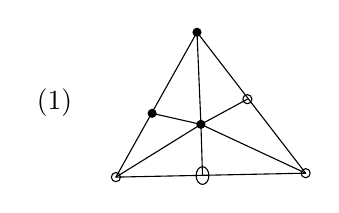
\begin{tikzpicture}[x=1cm,y=1cm,line cap=round,line join=round]
\coordinate (T) at (1.03,1.84);
\coordinate (L) at (0,0);
\coordinate (R) at (2.41,.05);
\coordinate (TL) at (.46,.81);
\coordinate (TR) at (1.67,.99);
\coordinate (B) at (1.1,.02);
\coordinate (C) at (1.08,.67);
\node[anchor=east] at (-.43,.95) {(1)};
\draw (L)--(T)--(R)--cycle;
\draw (T)--(C)--(B) (L)--(C)--(TR) (R)--(C)--(TL);
\foreach \point in {T,TL,C} \fill (\point) circle[radius=1.65pt];
\foreach \point in {L,R,TR} \draw (\point) circle[radius=1.65pt]; \draw (B) ellipse[x radius=2.3pt,y radius=3.2pt];
\end{tikzpicture}}\endgroup}\par\smallskip
Seven marked points and three interior lines are visible. The lower middle loop extends below the base. No separate line through the three points on the sides is visible.}
\end{GelfandAdjacentEvidence}
\begin{GelfandAdjacentEvidence}{GELFAND-P001230}{8}

(Fano config.)\qquad over \(\mathbb R,\mathbb Z\) is not realizable.

A faithful rep. of a lattice \(=\) a map from it
\begin{equation*}
a:\Gamma\longrightarrow\mathcal L(F^n)\quad\text{--- lattice of subspaces,}
\end{equation*}
such that
\begin{equation*}
\gamma_1<\gamma_2\ \Rightarrow\ a(\gamma_1)<a(\gamma_2)
\end{equation*}
and \(\sup\) is preserved

(1) is not realizable [crossed out] over \(\mathbb R\), but over \(\mathbb Z_2\) realiz..
\Unclear{GELFAND-P001230}{realization-cancel}{The crossed-out mark before “over” is illegible.}
\end{GelfandAdjacentEvidence}



\Needspace{7\baselineskip}
\begin{GelfandAdjacentEvidence}{GELFAND-P001231}{1}
\SourcePage{GELFAND-P001231}{unlabelled}
A faithful rep. exists for config. (1):
\begin{equation*}
?\qquad m=4,\quad E,\quad \underline F,\quad \underline{\mathbb R^6}
\end{equation*}
\EvidenceBlock{GELFAND-P001231}{opening-symbols}{The line with the question mark lists \(m=4\), \(E\), \(F\) and \(\mathbb R^6\) separately.}{Manuscript notation.}
\end{GelfandAdjacentEvidence}
\begin{GelfandAdjacentEvidence}{GELFAND-P001231}{2}


Realizability problem \(\Leftrightarrow\) problem of solving a system of algebraic inequalities.
\EvidenceBlock{GELFAND-P001231}{inequalities-reading}{The abbreviation after “algebraic” is «нер-в.» (ner-v., “inequalities”).}{Manuscript notation.}
\end{GelfandAdjacentEvidence}
\begin{GelfandAdjacentEvidence}{GELFAND-P001231}{3}


\uwave{Nontriv. work on lattices:} (according to Gelfand)
\EvidenceBlock{GELFAND-P001231}{lattice-heading}{The first abbreviation in the heading is «Нетрив.» (Netriv., “Nontriv.”).}{Manuscript notation.}
\end{GelfandAdjacentEvidence}
\begin{GelfandAdjacentEvidence}{GELFAND-P001231}{4}


Dedekind: invented it

Kurosh, Ore.

von Neumann;

Gelfand, Ponomarev:

[In the left margin: \uwave{Vershik's add.:}]
\uwave{Pudlák and Tůma} (Czechs): every finite lattice embeds into the partition lattice of a finite set (very difficult theorem).

(\(\inf\) and \(\sup\) --- [crossed out] intersection and union)
\Incomplete{GELFAND-P001231}{inf-sup-cancel}{The word after “inf and sup” is crossed out and undeciphered.}
\end{GelfandAdjacentEvidence}
\begin{GelfandAdjacentEvidence}{GELFAND-P001231}{5}


\(0\) --- partition into points.

\medskip
\underline{\underline{Feigin B.}}\qquad\underline{On strings} [crossed out] (continued).
\Unclear{GELFAND-P001231}{string-heading-cancel}{The crossed-out vertical mark after “On strings” is undeciphered.}
\end{GelfandAdjacentEvidence}
\begin{GelfandAdjacentEvidence}{GELFAND-P001231}{6}


\underline{Operator theory of strings.}

\underline{Dual amplitudes.} Consider a collision of particles

\SourceFigure{GELFAND-P001231}{scattering-diagram}{%
\par\smallskip
{\color{black}\begingroup\color{black}\GelfandFitDiagram{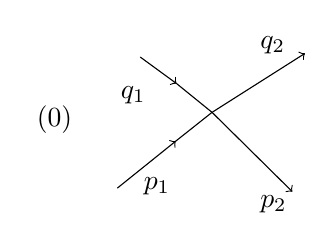
\begin{tikzpicture}[x=1cm,y=.96cm,line cap=round]
\node at (-2,0) {(0)};
\coordinate (lowerin) at (-1.2,-.90);
\coordinate (upperin) at (-.91,.83);
\coordinate (crossing) at (0,.10);
\coordinate (upperout) at (1.18,.88);
\coordinate (lowerout) at (1.02,-.95);
\draw[->] (lowerin)--(-.46,-.28);
\draw[->] (-.46,-.28)--(crossing)--(upperout);
\draw[->] (upperin)--(-.45,.48);
\draw[->] (-.45,.48)--(crossing)--(lowerout);
\node[below] at (-.70,-.63) {\(p_1\)};
\node[left] at (-.72,.33) {\(q_1\)};
\node[above] at (.77,.74) {\(q_2\)};
\node[below] at (.78,-.87) {\(p_2\)};
\end{tikzpicture}}\endgroup}\par\smallskip}
\end{GelfandAdjacentEvidence}
\begin{GelfandAdjacentEvidence}{GELFAND-P001231}{7}


Let the masses all be the same and the total momentum \(=0\)

All are vectors in space/time
\begin{equation*}
\begin{cases}
p_1+q_1=p_2+q_2,\\
p_1^2=q_1^2=p_2^2=q_2^2=m^2
\end{cases}
\qquad p_j,q_j\in\mathbb R^4.
\tag{1}
\end{equation*}
\EvidenceBlock{GELFAND-P001231}{mass-shell-overwrite}{The final form of the overwritten letter and its subscript in the penultimate square reads \(q_2\).}{Manuscript notation.}
\end{GelfandAdjacentEvidence}
\begin{GelfandAdjacentEvidence}{GELFAND-P001231}{8}


Let an \(S\)-matrix characterizing this collision be given,
\begin{equation*}
S(p_1,q_1,p_2,q_2)\tag{2}
\end{equation*}
Mandelstam variables:
\begin{equation*}
\begin{cases}
s=(p_1+q_1)^2,\\
t=(p_1-p_2)^2\\
u\ \text{[crossed out]}=(p_1-q_2)^2
\end{cases}\tag{3}
\end{equation*}
\Unclear{GELFAND-P001231}{mandelstam-u-cancel}{An illegible mark between \(u\) and the equals sign is crossed out.}
\end{GelfandAdjacentEvidence}
\begin{GelfandAdjacentEvidence}{GELFAND-P001231}{9}

[To the right of (3):] (Relativistically invariant pairwise scalar products are given)

dependent:
\begin{equation*}
s+t+u=4m^2\tag{4}
\end{equation*}
Define \(A(s,t)\) (\(=\) expression for \(S\) in terms of \(s,t\))

\uwave{Requirement}:
\begin{equation*}
1)\quad A\text{ is analytic in }s,t\quad\text{[crossed out]}\tag{5}
\end{equation*}
\Unclear{GELFAND-P001231}{analytic-tail}{A mark after \(t\) is crossed out. Its reading is unresolved.}
\end{GelfandAdjacentEvidence}



\Needspace{7\baselineskip}
\begin{GelfandAdjacentEvidence}{GELFAND-P001232}{1}
\SourcePage{GELFAND-P001232}{16}
2) \(A\) is symmetric in \(s,t\) (indep. of the order)

3) For fixed \(t\) the fn. \(A(s,t)\) has in \(s\) only simple poles,
and [inserted between words: 4)] the locations of the poles do not depend on \(t\). Usually one writes:
\begin{equation*}
A(s,t)=\sum_{n=0}^{\infty}\frac{R_n(t)}{n-\alpha(s)}\tag{6}
\end{equation*}
5) \(R_n(t)\) --- polynomial

The graph of \(\alpha(s)\) is called a Regge trajectory.

It turns out that from 1)---5) we uniquely determine the form of the fn. \(A\):
\begin{equation*}
A(s,t)=\frac{\Gamma(-\alpha(s))\Gamma(-\alpha(t))}{\Gamma(-\alpha(s)-\alpha(t))}
=B(-\alpha(s),-\alpha(t))\tag{7}
\end{equation*}
It follows from analysis of the exper. data that
\begin{equation*}
\alpha(s)\quad\text{--- linear fn.}\tag{8}
\end{equation*}
\(A\) is called the Veneziano amplitude, or dual amplitude, and conds. 1)---5) are called \underline{duality conditions}.

Operator method: we want to write \(A(s,t)\) as an operator expectation
\begin{equation*}
\langle0|V(t)V(s)|0\rangle,\tag{9}
\end{equation*}
where \(\langle0|\) --- vac. vector in some space, \(V(t)\) --- operators.

Another form of (7):
\begin{equation*}
S(p_1,p_2,p_3,p_4)=\int_0^1
x^{-2\langle p_1,p_2\rangle}(1-x)^{-2\langle p_2,p_3\rangle}
(x(1-x))^{-1-m^2}\,dx\tag{10}
\end{equation*}
Here

\SourceFigure{GELFAND-P001232}{amplitude-arrow-convention}{%
\par\smallskip
{\color{black}\begingroup\color{black}\GelfandFitDiagram{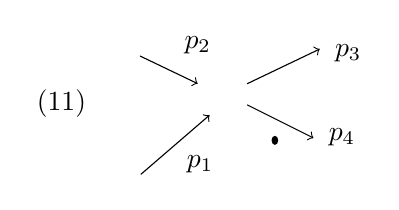
\begin{tikzpicture}[x=1cm,y=1cm,line cap=round]
\node at (-2.1,0) {(11)};
\draw[->] (-1.1,.60)--(-.37,.25);
\draw[->] (-1.09,-.90)--(-.22,-.15);
\draw[->] (.26,.25)--(1.18,.69);
\draw[->] (.26,-.02)--(1.1,-.44);
\node[above] at (-.37,.50) {\(p_2\)};
\node[below] at (-.34,-.54) {\(p_1\)};
\node[right] at (1.25,.64) {\(p_3\)};
\node[right] at (1.17,-.43) {\(p_4\)};
\fill (.61,-.47) ellipse[x radius=1.2pt,y radius=1.65pt];
\end{tikzpicture}}\endgroup}\par\smallskip
An ink mark is visible beside the lower-right arrow. Its relation to the arrow is unclear.}
\end{GelfandAdjacentEvidence}
\begin{GelfandAdjacentEvidence}{GELFAND-P001232}{2}

\begin{equation*}
p_1+p_2+p_3+p_4=0.
\end{equation*}
Similarly one can write amplitudes for a greater number of particles,
for example:
\begin{equation*}
A(p_1,p_2,p_3,p_4,p_5)\cong\int\int_0^1
x^{\cdots}y^{\cdots}(1-x)^{\cdots}(1-y)^{\cdots}(1-xy)^{\cdots}\,dx\,dy\tag{12}
\end{equation*}
This amplitude has not been calculated in general, only for some special values of the \underline{scalar products}.

The space is generated by a finite set of oscillators connected as in a string. A finite number will not do!.
\EvidenceBlock{GELFAND-P001232}{finite-oscillators}{The first sentence says “finite”. The second says “A finite number will not do!”}{Manuscript notation.}
\end{GelfandAdjacentEvidence}
\begin{GelfandAdjacentEvidence}{GELFAND-P001232}{3}


Consider the algebra with generators
\begin{equation*}
a_m^\mu,x^\mu,\quad \mu=0,1,\ldots,d,\quad
\text{[crossed out]}\tag{13}
\end{equation*}
\Incomplete{GELFAND-P001232}{generators-cancel}{The notation after \(d\) in (13) is crossed out and undeciphered.}
\end{GelfandAdjacentEvidence}

where \(d\) --- dim. of the space


\Needspace{7\baselineskip}
\begin{GelfandAdjacentEvidence}{GELFAND-P001233}{1}
\SourcePage{GELFAND-P001233}{unlabelled}
\begin{equation*}
\relax [a_m^\mu,a_n^\nu]=m g^{\mu\nu}\delta_{m,-n}\tag{14}
\end{equation*}
\(m,n\) --- integers
\begin{equation*}
a_0^\mu=p^\mu\tag{15}
\end{equation*}
\begin{equation*}
\relax [x^\mu,p^\nu]=i g^{\mu\nu}\tag{16}
\end{equation*}
\EvidenceBlock{GELFAND-P001233}{momentum-superscript}{The final form of the overwritten superscript on \(p\) in (16) reads \(\nu\).}{Manuscript notation.}
\end{GelfandAdjacentEvidence}
\begin{GelfandAdjacentEvidence}{GELFAND-P001233}{2}

\begin{equation*}
\relax [x^\mu,a_m^\nu]=0,\quad m\ne0\tag{17}
\end{equation*}
Meaning of the generators \(x^\mu,a_m^\mu\):

[Crossed out: \(p^\mu\) --- undeciphered]
\Unclear{GELFAND-P001233}{coordinates-cancel}{The crossed-out notation begins with \(p^\mu\). The remaining signs are illegible.}
\end{GelfandAdjacentEvidence}
\begin{GelfandAdjacentEvidence}{GELFAND-P001233}{3}

\((x^\mu,p^\mu)\) --- coord. and momentum of the center of gravity of the flying string, \(a_m^\mu\) --- Fourier series expansion of everything else.

Put:
\begin{equation*}
P^\mu(\theta)=\sum_{-\infty}^{+\infty}a_m^\mu e^{-im\theta},\tag{18}
\end{equation*}
(momentum of the point with param. \(\theta\))
\begin{equation*}
Q^\mu(\theta)=x^\mu+a_0^\mu\theta+
 i\sum_{\substack{n=-\infty\\n\ne0}}^{\infty}\frac1n a_{[m?]}^\mu e^{-in\theta}.\tag{19}
\end{equation*}
\Unclear{GELFAND-P001233}{fourier-index}{The overwritten subscript on \(a\) tentatively reads \(m\), with \(n\) also possible. The summation index and the index in the exponent are \(n\).}
\end{GelfandAdjacentEvidence}
\begin{GelfandAdjacentEvidence}{GELFAND-P001233}{4}

Then the commutation relations hold:
\begin{equation*}
\relax [Q_\mu(\theta),P_\nu(\theta')]=2\pi i g_{\mu\nu}\delta(\theta-\theta')\tag{20}
\end{equation*}
\begin{equation*}
\relax [P_\mu(\theta),P_\nu(\theta')]=2\pi i g_{\mu\nu}\delta'(\theta-\theta')\tag{21}
\end{equation*}
\begin{equation*}
\relax [Q_\mu(\theta),Q_\nu(\theta')]=-\pi i g_{\mu\nu}\varepsilon(\theta-\theta'),\tag{22}
\end{equation*}
where \(\varepsilon\) --- Heaviside fn.
\Unclear{GELFAND-P001233}{heaviside-convention}{The line reads “where \(\varepsilon\) is the Heaviside fn.” Its normalization is unspecified here.}
\end{GelfandAdjacentEvidence}
\begin{GelfandAdjacentEvidence}{GELFAND-P001233}{5}

\begin{equation*}
L_m\overset{\mathrm{def}}{=}\frac1{4\pi}\int_0^{2\pi}
e^{im\theta}:P^2(\theta):\,d\theta\tag{23}
\end{equation*}
Then one obtains a representation of the Virasoro algebra
\begin{equation*}
\relax [L_m,L_n]=(m-n)L_{m+n}+\frac d{12}(m^3-m)\delta_{m,-n}\tag{24}
\end{equation*}
\Unclear{GELFAND-P001233}{central-dimension}{The central coefficient is written \(\frac{d}{12}\).}
\end{GelfandAdjacentEvidence}


\uwave{Exercise}: verify this.

Incidentally,
\begin{equation*}
L_0=\frac12a_0^2+\sum_{n=1}^{\infty}a_{-n}a_n\tag{25}
\end{equation*}


\Needspace{7\baselineskip}
\begin{GelfandAdjacentEvidence}{GELFAND-P001234}{1}
\SourcePage{GELFAND-P001234}{17}
\begin{equation*}
2L_m={:}\sum_{r+s=m}a_ra_s{:}\tag{26}
\end{equation*}
\uwave{Vertex operator}: put
\begin{equation*}
V(k,\theta)=\exp\langle ik,Q(\theta)\rangle,\tag{27}
\end{equation*}
where \(k\) --- a vector, then
\begin{equation*}
V(k)=V(k,0)=
\exp\left\langle k,\sum_{n=1}^{\infty}\frac{a_{-n}}n\right\rangle
\exp(ikx)
\exp\left\langle-k,\sum_{n=1}^{\infty}\frac{a_n}n\right\rangle
\tag{28}
\end{equation*}
\EvidenceBlock{GELFAND-P001234}{vertex-insertion}{The factor \(\exp(ikx)\) is inserted above the line. The insertion strokes converge between the two exponentials.}{Manuscript notation.}
\end{GelfandAdjacentEvidence}
\begin{GelfandAdjacentEvidence}{GELFAND-P001234}{2}

and
\begin{equation*}
V(k,\theta)=\exp(i\theta L_0)V(k)\exp(-i\theta L_0).\tag{29}
\end{equation*}
Next,

[Crossed out before (30)]
\begin{equation*}
\relax [L_n-L_0,V(k)]=\frac{nk^2}2V(k).\tag{30}
\end{equation*}
\Incomplete{GELFAND-P001234}{commutator-cancel}{The notation before the commutator in (30) is crossed out and undeciphered.}
\end{GelfandAdjacentEvidence}
\begin{GelfandAdjacentEvidence}{GELFAND-P001234}{3}


Consider a series of interactions:

\SourceFigure{GELFAND-P001234}{interaction-chain}{%
\par\smallskip
{\color{black}\begingroup\color{black}\GelfandFitDiagram{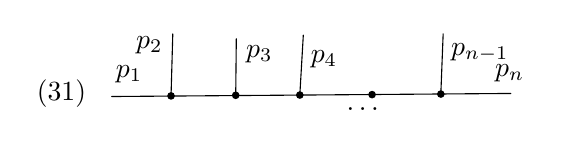
\begin{tikzpicture}[x=.74cm,y=.78cm,line cap=round]
\node at (-.86,.05) {(31)};
\draw (0,0)--(6.85,.05);
\draw (1.02,.01)--(1.05,1.02) (2.13,.02)--(2.14,.94)
      (3.23,.024)--(3.29,1.0) (5.65,.04)--(5.69,1.02);
\foreach \x/\y in {1.02/.01,2.13/.02,3.23/.024,4.47/.031,5.65/.04}
   \fill (\x,\y) circle[radius=1.38pt];
\node[above] at (.30,.06) {\(p_1\)};
\node[left] at (1.04,.83) {\(p_2\)};
\node[right] at (2.14,.69) {\(p_3\)};
\node[right] at (3.25,.61) {\(p_4\)};
\node[right] at (5.66,.72) {\(p_{n-1}\)};
\node[above] at (6.83,.08) {\(p_n\)};
\node[below] at (4.31,-.02) {\(\ldots\)};
\end{tikzpicture}}\endgroup}\par\smallskip}
\end{GelfandAdjacentEvidence}
\begin{GelfandAdjacentEvidence}{GELFAND-P001234}{4}


and from such a picture construct the amplitude:
\begin{equation*}
\langle0|V(p_2)D(s_2)V(p_3)D(s_3)\ldots D(s_{n-2})V(p_{n-1})|0\rangle,
\tag{32}
\end{equation*}
\EvidenceBlock{GELFAND-P001234}{last-propagator-index}{The overwritten numeral in the last argument of \(D\) reads \(2\). The argument is written \(s_{n-2}\).}{Manuscript notation.}
\end{GelfandAdjacentEvidence}

where \(p\) --- the same as \(k\),
\begin{equation*}
\begin{aligned}
s_2&=(p_2+p_1)^2\\
s_3&=(p_3+p_2+p_1)^2,\\
&\ldots
\end{aligned}\tag{33}
\end{equation*}
\begin{equation*}
D(s)=\int_0^1 x^{L_0-\alpha(s)-1}(1-x)^{\alpha(0)-1}\,dx,\tag{34}
\end{equation*}
where \(\alpha(s)\) --- linear fn. (Regge trajectory).

(32) --- dual amplitude. It should agree with \(A\), when there are 4 vertices.

Expand \(V(k,\theta)\) in a Fourier series:
\begin{equation*}
V(k,\theta)=\sum V_n(k)e^{-in\theta}.\tag{35}
\end{equation*}
There are operators \(a_i^\mu\) and \(a_0^\mu\) and vacuum vectors
\(|0,p\rangle\), satisfying the condition


\Needspace{7\baselineskip}
\begin{GelfandAdjacentEvidence}{GELFAND-P001235}{1}
\SourcePage{GELFAND-P001235}{unlabelled}
\begin{equation*}
a_i^\mu|0,p\rangle=0,\quad\text{if }i>0,
\tag*{$(36)_i$}
\end{equation*}
\begin{equation*}
a_0^\mu|0,p\rangle=
\text{[crossed out]}\ p^\mu\,\text{[crossed out]}\ |0,p\rangle.
\tag*{$(36)_0$}
\end{equation*}
\Unclear{GELFAND-P001235}{vacuum-cancel-left}{crossed-out writing before $p^\mu$}
\end{GelfandAdjacentEvidence}
\begin{GelfandAdjacentEvidence}{GELFAND-P001235}{2}

\Unclear{GELFAND-P001235}{vacuum-cancel-right}{crossed-out sign after $p^\mu$}
\end{GelfandAdjacentEvidence}
\begin{GelfandAdjacentEvidence}{GELFAND-P001235}{3}

(the vacua are indexed by momentum vectors)

We obtain the space
\begin{equation*}
\bigoplus_p H(p)
\tag{37}
\end{equation*}
The vertex operator acts as follows:
\begin{equation*}
V_n(k):H(p)\longrightarrow H(p+k).
\tag{38}
\end{equation*}
Commutation relations:

[Crossed out: illegible]
\Incomplete{GELFAND-P001235}{commutator-cancel}{The crossed-out writing under “Commutation relations” is illegible.}
\end{GelfandAdjacentEvidence}
\begin{GelfandAdjacentEvidence}{GELFAND-P001235}{4}

\begin{equation*}
\relax [a_m^\mu,V_n(k)]=V_{n+m}(k)\cdot k_\mu
\tag{39}
\end{equation*}
\EvidenceBlock{GELFAND-P001235}{commutator-index}{In the factor \(k_\mu\) in (39), \(\mu\) is written below the baseline.}{Manuscript notation.}
\end{GelfandAdjacentEvidence}
\begin{GelfandAdjacentEvidence}{GELFAND-P001235}{5}


[Crossed out: $V_n(k_1)|0,p\rangle$ / $V_1(k_1)|0,p\rangle$\textsuperscript{?}] Set
\Unclear{GELFAND-P001235}{vertex-cancel}{The crossed-out expression shows \(V\), \((k_1)\) and \(\lvert 0,p\rangle\). The subscript on \(V\) may be \(n\) or \(1\).}
\end{GelfandAdjacentEvidence}
\begin{GelfandAdjacentEvidence}{GELFAND-P001235}{6}

\begin{equation*}
\langle0,p+k_1+k|V_{-n}(k_2)V_n(k_1)|0,p\rangle=A_n\qquad\text{(these are numbers)}
\tag{40}
\end{equation*}
\EvidenceBlock{GELFAND-P001235}{bra-last-momentum}{The bra in (40) has \(p+k_1+k\). The final \(k\) has no written subscript.}{Manuscript notation.}
\end{GelfandAdjacentEvidence}


Then
\begin{equation*}
\sum A_n z^n=(1-z)^{\langle k_1,k_2\rangle}.
\tag{41}
\end{equation*}
This follows by a direct computation. The reader is asked to verify (41) as an exercise.


\Needspace{7\baselineskip}
\begin{GelfandAdjacentEvidence}{GELFAND-P001236}{1}
\SourcePage{GELFAND-P001236}{26}
\underline{18 Nov. 1985}\qquad \underline{Gelfand Seminar}

\underline{B. Feigin} (continued).

The $L_i$ generate the Virasoro algebra. Let there be a large space on which this algebra acts.

Eigenvectors of $L_0$ are weight vectors.

By the commutation relations, $L_i$ acts on the space of weight vectors.

(see (24) on p.~17, left)

Highest [crossed out: vector?\textsuperscript{?}] weight: a vector that cannot be raised any further
\Unclear{GELFAND-P001236}{highest-cancel}{The crossed-out word may read «вектор» (vektor, “vector”). The strokes obscure the middle of the word.}
\end{GelfandAdjacentEvidence}
\begin{GelfandAdjacentEvidence}{GELFAND-P001236}{2}

\begin{equation*}
\widetilde{\mathcal H}=\{v\mid L_0v=v,\quad L_iv=0\ \text{for }i>0\}.\qquad\text{(weight 1)}
\tag{1}
\end{equation*}
\begin{equation*}
\overline{\mathcal H}=\{v\in\widetilde{\mathcal H},\quad v=L_i v',\ i<0\},
\tag{2}
\end{equation*}
[At right:] Here $v'$ is an arbitrary weight vector from the large space.

(the space of “spurions,” a term used by physicists some 15 years ago)
\begin{equation*}
\mathcal H\overset{\mathrm{def}}{=}\widetilde{\mathcal H}/\overline{\mathcal H}
\tag{3}
\end{equation*}
\begin{equation*}
\prod_{i=1}^N a_{m_i}^{\mu_i}|0,p\rangle
\tag{4}
\end{equation*}
[At right:] (space of states)

a large module over the Virasoro algebra
\begin{equation*}
L_{-1}v'=v\quad\Rightarrow\quad v'\text{ has weight }2:\quad L_0v'=2v'
\tag{5}
\end{equation*}
\EvidenceBlock{GELFAND-P001236}{weight-two}{In (5) the manuscript has \(L_{-1}v'=v\), “\(v'\) has weight 2” and \(L_0v'=2v'\).}{Manuscript notation.}
\end{GelfandAdjacentEvidence}
\begin{GelfandAdjacentEvidence}{GELFAND-P001236}{3}


The aim is to quotient by the diffeomorphism group throughout the space, but a central extension acts, and the centre acts nontrivially.

Another procedure is proposed for obtaining “invariant” vectors. They are invariant under one half, then we quotient by the action of the others and discard them.

The Virasoro algebra disappears, leaving the space of invariants.

We want to

I. Construct a space generated by $d-2$ oscillators.

II. Prove that all vectors in $\widetilde{\mathcal H}/\overline{\mathcal H}$ have norm $>0$.

(this does not hold in the original $d$-dimensional space)

(absence of \underline{tachyons\textsuperscript{?}})
\EvidenceBlock{GELFAND-P001236}{tachyon-word}{The underlined word reads «тахионов» (takhionov, “tachyons”).}{Manuscript notation.}
\end{GelfandAdjacentEvidence}


All of this is achieved in dimension 26.


\Needspace{7\baselineskip}
\begin{GelfandAdjacentEvidence}{GELFAND-P001237}{1}
\SourcePage{GELFAND-P001237}{unlabelled}
Vertex operators
\begin{equation*}
X(p,z)=\exp\left(p_\mu\cdot\sum_{n=1}^{\infty}a_{-n}^\mu z^n\right)D_p
\exp\left(-p_\mu\sum_{n=1}^{\infty}\frac{a_n^\mu}{n}z^{-n}\right),
\tag{6}
\end{equation*}
\EvidenceBlock{GELFAND-P001237}{left-exponential-normalization}{The left exponential in (6) has \(a_{-n}^{\mu}z^n\), with no fraction bar or denominator.}{Manuscript notation.}
\end{GelfandAdjacentEvidence}
\begin{GelfandAdjacentEvidence}{GELFAND-P001237}{2}


where the operators $D_p$ are defined by the formulas
\begin{equation*}
D_p|0,k\rangle=|0,k+p\rangle,\quad [D_p,a_n^\mu]=0,\ n\ne0.
\tag{7}
\end{equation*}
Correlation function
\begin{equation*}
\begin{aligned}
&\langle0,k+\textstyle\sum p_i|X(z_1,p_1)\ldots X(z_n,p_n)|0,k\rangle\\
&\qquad=\prod_{j>1}\left(1-\frac{z_j}{z_i}\right)^{\langle p_i,p_j\rangle}.
\end{aligned}
\tag{8}
\end{equation*}
\EvidenceBlock{GELFAND-P001237}{product-index}{The index under the product is \(j>1\). The final sign has the baseline foot of the numeral \(1\).}{Manuscript notation.}
\end{GelfandAdjacentEvidence}
\begin{GelfandAdjacentEvidence}{GELFAND-P001237}{3}


Expanding $X(z,p)$ in a series gives
\begin{equation*}
X(z,p)=\sum X_i(p)z^i
\tag{9}
\end{equation*}
(this defines the operators $X_i(p)$)

We want to construct 24 oscillators.

Next we will construct the operators
\begin{equation*}
\int X(p,z)\frac{dz}{z},
\tag{10}
\end{equation*}
which commute with the Virasoro algebra when $\langle p,p\rangle=2$.
\begin{equation*}
\begin{aligned}
&\text{In }\mathbb R^{26}\text{ we want to have }p_1,\ldots,p_n:\quad\langle p_i,p_i\rangle=2\\
&\langle p_i,p_j\rangle=A_{ij}\in\mathbb Z,\quad A_{ij}<0.
\end{aligned}
\tag{11}
\end{equation*}
[In the left margin: crossed-out vertical sign\textsuperscript{?}]
\Unclear{GELFAND-P001237}{cartan-margin-cancel}{crossed-out vertical sign}
\end{GelfandAdjacentEvidence}
\begin{GelfandAdjacentEvidence}{GELFAND-P001237}{4}


\EvidenceBlock{GELFAND-P001237}{cartan-diagonal}{The manuscript has \(A_{ij}<0\). There is no index restriction written beside the inequality.}{Manuscript notation.}
\end{GelfandAdjacentEvidence}


Then the operators
\begin{equation*}
e_i=\int X(p_i,z)\frac{dz}{z},\quad f_i=\int X(-p_i,z)\frac{dz}{z}
\tag{12}
\end{equation*}
generate an action of the Kac–Moody algebra with Cartan matrix $A_{ij}$ on the space. We must also set
\begin{equation*}
h_i|0,k\rangle=\langle k,p_i\rangle|0,k\rangle
\tag{13}
\end{equation*}
\underline{Read} the \underline{article by Macdonald} (the beginning), \underline{Sem. Bourbaki}.

Use it to study Lie algebras.

[In the left margin: I.M.G.] The largest finite simple group has $\sim10^{54}$ elements. It is related to strings!

[Added at right:] (Monster “Moonshine”)

Moonshine

(there is work by Frenkel, Lepowsky and someone else)

Somehow one obtains a fundamental representation of the Kac–Moody algebra.


\Needspace{7\baselineskip}
\begin{GelfandAdjacentEvidence}{GELFAND-P001238}{1}
\SourcePage{GELFAND-P001238}{27}
In $\mathbb R^{26}$ consider the metric $\langle-1,1,1,\ldots,1\rangle$,

[Crossed out: nulev…?] vector of length 0, [crossed out: illegible]
\Unclear{GELFAND-P001238}{null-cancel-before}{The crossed-out fragment tentatively reads «нулев…» (nulev…). The ending is illegible.}
\end{GelfandAdjacentEvidence}
\begin{GelfandAdjacentEvidence}{GELFAND-P001238}{2}

\Incomplete{GELFAND-P001238}{null-cancel-after}{The crossed-out word after “vector of length 0” is illegible.}
\end{GelfandAdjacentEvidence}
\begin{GelfandAdjacentEvidence}{GELFAND-P001238}{3}


[Before the next line: two vertical marks, the right one resembling a brace\textsuperscript{?}] 24 oscillators
\Unclear{GELFAND-P001238}{null-marks}{Two separated vertical marks are visible. The right one resembles a brace with a lower hook. Their function is unclear.}
\end{GelfandAdjacentEvidence}
\begin{GelfandAdjacentEvidence}{GELFAND-P001238}{4}


(Review by D. (?) Schwarz, 1973).
\Unclear{GELFAND-P001238}{schwarz-initial}{A rounded sign, tentatively D., is visible beside vertical strokes before “Schwarz”. The initial remains uncertain.}
\end{GelfandAdjacentEvidence}


\begin{center}—\quad .\quad —\end{center}

Take $\mathbb R^d$ with an indefinite metric and a given vector $p$ with $\langle p,p\rangle=0$.

[Under “metric”:] (Minkowski, one minus sign)

Set
\begin{equation*}
U_n(v)=\int v(z)X(np,z)\frac{dz}{z},
\tag{14}
\end{equation*}
where $v\in\mathbb R^d$, $v=\sum v_i e_i$, $v(z)=\sum v_\mu a_n^\mu z^n$

Let
\begin{equation*}
v^1,v^2,\ldots,v^{d-2}\text{ be such that }\langle v^i,p\rangle=0
\tag{15}
\end{equation*}
\begin{GelfandAdjacentEvidence}{GELFAND-P001238}{5}
[“and” inserted over the crossed-out sign:] and [crossed out: crossed-out sign under the inserted “and”\textsuperscript{?}]
\Unclear{GELFAND-P001238}{basis-cancel-left}{«и» (“and”) is inserted above the crossing-out. The cancelled sign is illegible.}
\end{GelfandAdjacentEvidence}
\begin{GelfandAdjacentEvidence}{GELFAND-P001238}{6}

$v^1,v^2,\ldots,v^{d-2},p$ are a basis of the space
[crossed out: illegible] $\{x:\langle x,p\rangle=0\}$.
\Unclear{GELFAND-P001238}{basis-cancel-right}{The crossed-out word after “in the space” may begin with «в» (v). The remaining letters are illegible.}
\end{GelfandAdjacentEvidence}
\begin{GelfandAdjacentEvidence}{GELFAND-P001238}{7}


Set
\begin{equation*}
b_n^\mu=U_n(v^\mu);
\tag{16}
\end{equation*}
The $b_n^\mu$ form a Heisenberg algebra $\Rightarrow$ oscillators.

They generate the whole space.

There is also a review by Green and Schwarz (a volume of Physics Reports).

\bigskip
\underline{A. Zelevinsky}\qquad \underline{Schubert cells}
[inserted above the line: \underline{(and polynomials)}]
\underline{and the cohomology of flag varieties.}

On the work of \underline{A. [crossed out: illegible mark] Lascoux}, \underline{M.-P. Schützenberger}
\Unclear{GELFAND-P001238}{lascoux-cancel}{An illegible crossed-out mark, possibly a letter or initial, appears between “A.” and “Lascoux”.}
\end{GelfandAdjacentEvidence}
\begin{GelfandAdjacentEvidence}{GELFAND-P001238}{8}


(Schubert cells and the cohomology of Grassmannians and flag varieties)

Continuation of work by Bernstein, I.M.G. and S.I.G., Uspekhi Mat. Nauk, 1973, 28(3), 3–26.

$X$ is the set of complete flags in $V^n$ (flags of subspaces).

[Below $X$, above (1): $\Vert$ (?), two vertical strokes]
\Unclear{GELFAND-P001238}{flag-relation}{Two vertical strokes appear below \(X\), tentatively \(\Vert\). Between them is a fine transverse trace aligned with the paper ruling. The function of the sign is unclear.}
\end{GelfandAdjacentEvidence}

\begin{equation*}
\{V^1\subset V^2\subset\ldots\subset V^n\}
\tag{1}
\end{equation*}
The cohomology is described in two ways.

$1^{\circ}.$ \underline{Borel}
\begin{equation*}
H^*(X,\mathbb Q)=\mathbb Q[x_1,\ldots,x_n]/J
\end{equation*}
The ideal $J$ is generated by symmetric polynomials with zero constant term.

$2^{\circ}.$ The Schubert cells $(c_w)$ form a basis in homology $H_*(X,\mathbb Q)$.
\nopagebreak[4]
$w$ is a permutation of the numbers from 1 to $n$.


\Needspace{7\baselineskip}
\begin{GelfandAdjacentEvidence}{GELFAND-P001239}{1}
\SourcePage{GELFAND-P001239}{unlabelled}
\begin{equation*}
\begin{array}{cccc}
1&2&\ldots&n\\
i_1&i_2&\ldots&i_n
\end{array}
\end{equation*}
Consider a fixed complete flag
\begin{equation*}
F=(\langle e_1\rangle,\ \langle e_1,e_2\rangle,\ \langle e_1,e_2,e_3\rangle,\ldots,\ \langle e_1,e_2,\ldots,e_n\rangle).
\end{equation*}
Act on it by the permutation $w$
\begin{equation*}
F_w=(\langle e_{w(1)}\rangle,\ \langle e_{w(1)},e_{w(2)}\rangle,\ldots)
=(\langle e_{i_1}\rangle,\ \langle e_{i_1},e_{i_2}\rangle,\ldots).
\end{equation*}
[Crossed out: [Kletka?]. Inserted above the crossing-out: $(C_w)\overset{\mathrm{def}}{=}$.]
\Unclear{GELFAND-P001239}{cancel-cell}{The initial stroke resembles «К» (K). The crossed-out word tentatively reads «Клетка» (Kletka). The remaining letters are illegible.}
\end{GelfandAdjacentEvidence}
\begin{GelfandAdjacentEvidence}{GELFAND-P001239}{2}

[Underlined: (Orbit of the flag $F_w$ under the linear transformations preserving $F$).]
[Crossed out: illegible notation\textsuperscript{?}.]
\Unclear{GELFAND-P001239}{cancel-after-orbit}{illegible notation}
\end{GelfandAdjacentEvidence}
\begin{GelfandAdjacentEvidence}{GELFAND-P001239}{3}

\begin{equation*}
\dim_{\mathbb C} c_w=\ell(w)\text{ is the number of inversions in }w.
\end{equation*}
The dual basis in cohomology
\begin{equation*}
P_w\in H^{2\ell(w)}(X;\mathbb Q).
\end{equation*}
B.–G.–G. found explicit formulas for $P_w$ in the Borel presentation, polynomials (!).
[Under the first occurrence of “polynomials”: $(\operatorname{mod}J)$.]
[Crossed out: illegible\textsuperscript{?}.]
\Unclear{GELFAND-P001239}{middle-cancel}{illegible}
\end{GelfandAdjacentEvidence}
\begin{GelfandAdjacentEvidence}{GELFAND-P001239}{4}

They have now been lifted to actual polynomials. Their degrees are
\begin{equation*}
\operatorname{deg} P_w=\ell(w).
\end{equation*}
\begin{equation*}
P_{\mathrm{id}}=1.
\end{equation*}
\begin{equation*}
w_0=(n,n-1,\ldots,1).
\end{equation*}
Then
\begin{equation*}
\operatorname{deg} P_{w_0}=\frac{n(n-1)}{2}.
\end{equation*}
The choice is nonunique. Take
\begin{equation*}
P_{w_0}=x_1^{n-1}x_2^{n-2}\ldots x_{n-1}.
\end{equation*}
(In B.–G.–G. $\displaystyle\prod_{i<j}(x_i-x_j)$ is the same modulo the ideal.)
\EvidenceBlock{GELFAND-P001239}{bgg-normalization}{No normalization factor is written before the product over \(i<j\).}{Manuscript notation.}
\end{GelfandAdjacentEvidence}
\begin{GelfandAdjacentEvidence}{GELFAND-P001239}{5}


Or $\displaystyle\frac{\rho^{m(n-1)/2}}{\left(\frac{m(n-1)}{2}\right)!}$, where $\rho=(n-1)x_1+(n-2)x_2+\ldots$
\EvidenceBlock{GELFAND-P001239}{rho-degree}{Both in the exponent on \(\rho\) and below the fraction bar, \(m\) precedes \((n-1)\).}{Manuscript notation.}
\end{GelfandAdjacentEvidence}


The rest are given by
\begin{equation*}
P_w=A_{w_0w^{-1}}P_{w_0},
\end{equation*}


\Needspace{7\baselineskip}
\begin{GelfandAdjacentEvidence}{GELFAND-P001240}{1}
\SourcePage{GELFAND-P001240}{28}
$A_w$ is the operator corresponding to the permutation
\begin{equation*}
w=(i_1,i_1+1)(i_2,i_2+1)\ldots(i_{\ell(w)},i_{\ell(w)+1})
\end{equation*}
(a product of inversions).
\EvidenceBlock{GELFAND-P001240}{top-last-index}{In the second index of the last transposition, \(+1\) is at the height of \(\ell(w)\), giving \(i_{\ell(w)+1}\).}{Manuscript notation.}
\end{GelfandAdjacentEvidence}
\begin{GelfandAdjacentEvidence}{GELFAND-P001240}{2}


\begin{equation*}
A_{(i,i+1)}=
\frac{p(x_1,\ldots,x_i,x_{i+1},\ldots,x_n)-p(x_1,\ldots,x_{i+1},x_i,\ldots,x_n)}{x_{i+1}-x_i}.
\end{equation*}
[Crossed out after the equals sign, before the fraction: $p(x_1,\ldots$; the rest is illegible.]
\Unclear{GELFAND-P001240}{cancel-polynomial}{The crossed-out expression begins \(p(x_1,\ldots\). A later stroke resembles \(x\). The final indices and parentheses are illegible.}
\end{GelfandAdjacentEvidence}
\begin{GelfandAdjacentEvidence}{GELFAND-P001240}{3}

\EvidenceBlock{GELFAND-P001240}{fraction-sign}{The denominator reads \(x_{i+1}-x_i\).}{Manuscript notation.}
\end{GelfandAdjacentEvidence}
\begin{GelfandAdjacentEvidence}{GELFAND-P001240}{4}


The operator
\begin{equation*}
A_w=A_{(i_1,i_1+1)}\ldots A_{(i_{\ell(w)},i_{\ell(w)+1})}
\end{equation*}
\EvidenceBlock{GELFAND-P001240}{operator-last-index}{In the second index of the last operator factor, \(+1\) is at the height of \(\ell(w)\).}{Manuscript notation.}
\end{GelfandAdjacentEvidence}


is well defined (independent of the decomposition into a product of inversions).
This is the operator used in the formula.

\underline{Symmetry condition}.

$P_w$ is symmetric in $x_i,x_{i+1}$ if $(i,i+1)$ is not an inversion of $w$.


\Needspace{7\baselineskip}
\begin{GelfandAdjacentEvidence}{GELFAND-P001241}{1}
\SourcePage{GELFAND-P001241}{35}
\underline{25 Nov. 1985}\qquad \underline{Gelfand Seminar.}

\underline{Feigin} (continued). (On strings).

Generators of the Virasoro algebra
\begin{equation*}
L_i=:\sum_{m+n=i}g_{\mu\nu}a_m^\mu a_n^\nu:\tag{1}
\end{equation*}
\EvidenceBlock{GELFAND-P001241}{normal-order-normalization}{The opening colon is followed directly by the summation sign, with \(m+n=i\) below it.}{Manuscript notation.}
\end{GelfandAdjacentEvidence}
\begin{GelfandAdjacentEvidence}{GELFAND-P001241}{2}


The colons $:\quad:$ make the operator well defined and only add a constant.

\underline{I.M.G.} What is required for the operation $:\quad:$ to exist? Here it gives rise to the Virasoro algebra. What if we take a lattice or a torus? What happens on the sphere?
\begin{equation*}
\relax [L_i,L_j]=(i-j)L_{i+j}+\delta_{i,-j}\frac{i^3-i}{12}\,c\tag{2}
\end{equation*}
\begin{equation*}
p^\mu(t)=\sum a_m^\mu e^{-imt},\qquad
q^\mu(t)=\sum_{m\ne0}\frac{a_m^\mu}{m}e^{-imt}+q_0^\mu\tag{3}
\end{equation*}
\begin{align*}
[x^\mu,a_m^\nu]&=0,\quad m\ne0,\\[0pt]
[x^\mu,a_0^\nu]&=g^{\mu\nu},\\
x^\mu(t)&=x^\mu+\sum_{n\ne0}\frac1n\bigl(a_n^\mu e^{-int}\bigr).
\end{align*}
\underline{I.M.G.} In the classical theory
\begin{equation*}
L_n=e^{int}\frac{d}{dt}.
\end{equation*}
Quantum mechanics corresponds to a one-dimensional extension of the classical theory. Compare $[\frac{d}{dx},x]=1$.

(4) $\mathcal H_p$ is the module generated by the highest vector $|p\rangle$.

[At right: ([crossed out] $a_m^\mu$ etc.). “(apply)” is inserted above the crossed-out sign, with a line to the insertion point.]
\Unclear{GELFAND-P001241}{module-margin}{The crossed-out notation before \(a_m^\mu\) is illegible. The insertion «(примен.)» (primen.) is linked to it.}
\end{GelfandAdjacentEvidence}
\begin{GelfandAdjacentEvidence}{GELFAND-P001241}{3}


[Between the lines:] This is a module over the Virasoro algebra.

(5) Its structure [crossed out] depends only on $\langle p,\ [\text{illegible}]\ p\rangle$; by definition
\Unclear{GELFAND-P001241}{depends-cancel}{small crossed-out sign before “depends”}
\end{GelfandAdjacentEvidence}
\begin{GelfandAdjacentEvidence}{GELFAND-P001241}{4}

\Unclear{GELFAND-P001241}{module-norm}{The overwritten sign between the comma and the second \(p\) resembles \(\xi\). Its reading and status are unclear.}
\end{GelfandAdjacentEvidence}


\begin{equation*}
a_m^\nu|p\rangle=0,\quad m>0,\qquad
 a_0^\nu|p\rangle=p^\nu|p\rangle\tag{6}
\end{equation*}
(5) $\mathcal H_p\cong\mathcal H_{p'}$, if $\langle p,p\rangle=\langle p',p'\rangle$.
$\Vert$ Denote it by $\mathcal H_{\langle p,p\rangle}$.

Consider
\begin{equation*}
\bigoplus_{\langle p,p\rangle\in\mathbb R}\mathcal H_{\langle p,p\rangle}\tag{7}
\end{equation*}


\Needspace{7\baselineskip}
\begin{GelfandAdjacentEvidence}{GELFAND-P001242}{1}
\SourcePage{GELFAND-P001242}{unlabelled}
Define the space of physical states from [crossed out] module (7), as was done [crossed out] above (p. (26)).
\Unclear{GELFAND-P001242}{cancel-before-module}{illegible crossed-out sign before “module”}
\end{GelfandAdjacentEvidence}
\begin{GelfandAdjacentEvidence}{GELFAND-P001242}{2}

\Unclear{GELFAND-P001242}{cancel-before-above}{illegible crossed-out sign before “above”}
\end{GelfandAdjacentEvidence}
\begin{GelfandAdjacentEvidence}{GELFAND-P001242}{3}


The construction depends [inserted above the line: only] on the [crossed out] action of the Virasoro algebra.
\Unclear{GELFAND-P001242}{cancel-before-action}{The crossed-out word before “action” tentatively reads «определения» (opredeleniia). Its middle letters are obscured.}
\end{GelfandAdjacentEvidence}
\begin{GelfandAdjacentEvidence}{GELFAND-P001242}{4}


(8) \underline{Theorem}. (on ghosts).

1) There is a system of oscillators $b_m^\mu$, $m\ne0$, $\mu=1,2,\ldots,24$
with standard commutation relations [undeciphered sign] on the space of [crossed out, inserted above the line: physical states], such that
\Unclear{GELFAND-P001242}{oscillator-prefix}{The separate tall looped mark may read «д» (d). Its expansion is unclear.}
\end{GelfandAdjacentEvidence}
\begin{GelfandAdjacentEvidence}{GELFAND-P001242}{5}

\Unclear{GELFAND-P001242}{cancel-physical-space}{illegible crossed-out notation beneath the insertion “physical states”}
\end{GelfandAdjacentEvidence}
\begin{GelfandAdjacentEvidence}{GELFAND-P001242}{6}

\begin{equation*}
\relax [L_i,b_m^\mu]=0.
\end{equation*}
The $b_m^\mu$ can be constructed from $a$.

2) $\exists$ a vacuum vector in the space of physical states [inserted above: $\widetilde{\mathcal H}$] $|0\rangle$,
and $\widetilde{\mathcal H}$ is generated by the vectors $|0\rangle$ and the operators $b_n^\nu$.
This holds only for \underline{\underline{$d=26$}}.

3) In $\widetilde{\mathcal H}$ there is a natural quadratic form inherited from space (7). It is positive definite on $\widetilde{\mathcal H}$.
\begin{equation*}
X(p,z)=\exp\left(p_\mu\sum_{n=1}^{\infty}\frac{a_{-n}^\mu}{n}z^n\right)
D_p\exp\left(-p_\mu\sum_{n=1}^{\infty}\frac{a_n^\mu}{n}z^{-n}\right),\tag{9}
\end{equation*}
Here $D_p$ is defined by the formula
\begin{equation*}
D_p|k\rangle=|k+p\rangle,\tag{10}
\end{equation*}
[Crossed out: and in this case.] Moreover
\begin{equation*}
\relax [D_p,a_n^\mu]=0,\quad n\ne0.\tag{11}
\end{equation*}
Commutation relations for $X(p,z)$ and $a_n^\mu$. If
\begin{equation*}
X(p,z)=\sum X_j(p)z^j,
\end{equation*}
then
\begin{equation*}
\relax [a_n^\mu,X_i(p)]=p^\mu X_{i+n}(p).\tag{12}
\end{equation*}
\EvidenceBlock{GELFAND-P001242}{mode-convention}{The expansion has \(z^j\). The right-hand side of (12) has \(X_{i+n}(p)\).}{Manuscript notation.}
\end{GelfandAdjacentEvidence}
\begin{GelfandAdjacentEvidence}{GELFAND-P001242}{7}


\underline{Representation of the current algebra.}

A space of dimension $d$. In $\mathbb R^d$ consider a lattice $Q$ (a discrete subgroup). Assume that $Q$ is integral and unimodular, so there is a basis
\begin{equation*}
e_1,\ldots,e_d,\quad\text{such that }\langle e_i,e_j\rangle\text{ is integral and }\det\langle e_i,e_j\rangle=1.\tag{13}
\end{equation*}
Even lattice
\begin{equation*}
\forall\gamma\in Q:\quad\langle\gamma,\gamma\rangle\text{ is even}.\tag{14}
\end{equation*}

[Narrow strip of the adjacent leaf at the right edge of the frame.]
\Unclear{GELFAND-P001242}{right-edge}{From top to bottom, four clipped opening parentheses, a short vertical stroke and one more opening parenthesis are visible. Their contents are outside the frame.}
\end{GelfandAdjacentEvidence}



\Needspace{7\baselineskip}
\begin{GelfandAdjacentEvidence}{GELFAND-P001243}{1}
\SourcePage{GELFAND-P001243}{36}
(15) \underline{Root of a lattice} is a vector $\gamma\in Q$, such that $\langle\gamma,\gamma\rangle=2$.

(16) [Crossed out] Such lattices occur from dimension [crossed out] $8$ [crossed out], more precisely,
[crossed out] only in dimensions divisible by $8$.
\Unclear{GELFAND-P001243}{cancel-before-these}{illegible crossed-out mark after (16)}
\end{GelfandAdjacentEvidence}
\begin{GelfandAdjacentEvidence}{GELFAND-P001243}{2}

\Unclear{GELFAND-P001243}{cancel-before-eight}{illegible crossed-out sign before $8$}
\end{GelfandAdjacentEvidence}
\begin{GelfandAdjacentEvidence}{GELFAND-P001243}{3}

\Unclear{GELFAND-P001243}{cancel-after-eight}{illegible crossed-out sign after $8$}
\end{GelfandAdjacentEvidence}
\begin{GelfandAdjacentEvidence}{GELFAND-P001243}{4}

\Unclear{GELFAND-P001243}{cancel-before-only}{illegible crossed-out sign before “only”}
\end{GelfandAdjacentEvidence}
\begin{GelfandAdjacentEvidence}{GELFAND-P001243}{5}


\underline{Exercise} Construct \underline{such} a lattice in $\mathbb R^8$.

\begin{center}—\quad .\quad —\end{center}

$Q$ is a lattice (for now, it need not be even).

\underline{Incidentally} [Crossed out] The root lattices of groups in series $A,D,E$ have property (14).
\Unclear{GELFAND-P001243}{aside-cancel}{crossed-out sign before “root lattices”}
\end{GelfandAdjacentEvidence}
\begin{GelfandAdjacentEvidence}{GELFAND-P001243}{6}


Consider the function
\begin{equation*}
\varepsilon:Q\times Q\longrightarrow\{\pm1\}\tag{17}
\end{equation*}
\begin{equation*}
\varepsilon(\alpha,\beta)\cdot\varepsilon(\beta,\alpha)=(-1)^{\langle\alpha,\beta\rangle},
\qquad\alpha,\beta\in Q;\tag{18}
\end{equation*}
\EvidenceBlock{GELFAND-P001243}{epsilon-parity}{The equality in (18) is followed by \(\alpha,\beta\in Q\).}{Manuscript notation.}
\end{GelfandAdjacentEvidence}
\begin{GelfandAdjacentEvidence}{GELFAND-P001243}{7}

\begin{equation*}
\varepsilon(\alpha,\alpha)=-1\quad\text{if }\langle\alpha,\alpha\rangle=2.\tag{19}
\end{equation*}
$\Delta$ is the set of roots of the lattice $Q$, i.e.
$\Delta=\{\gamma\in Q\mid\langle\gamma,\gamma\rangle=2\}$.

Let the quadratic form $\langle\ ,\ \rangle$ be positive definite.
Introduce the Lie algebra
\begin{equation*}
\mathfrak g=f+\sum_{\alpha\in\Delta}\mathbb Cx_\alpha,\tag{20}
\end{equation*}
where $f=\mathbb R^d\otimes\mathbb C=\mathbb C^d$.
\Unclear{GELFAND-P001243}{cartan-symbol}{Both looped signs have the written form of \(f\). The intended symbol is unclear.}
\end{GelfandAdjacentEvidence}
\begin{GelfandAdjacentEvidence}{GELFAND-P001243}{8}


Define the Lie algebra structure on $\mathfrak g$ by the formulas
\begin{equation*}
\relax [h,x_\alpha]=\langle h,\alpha\rangle x_\alpha;\tag*{$(21)_1$}
\end{equation*}
\begin{equation*}
\relax [x_\alpha,x_\beta]=0\quad\text{if }\alpha+\beta\notin\Delta\cup\{0\};\tag*{$(21)_2$}
\end{equation*}
\begin{equation*}
\relax [x_\alpha,x_\beta]=\varepsilon(\alpha,\beta)x_{\alpha+\beta}
\quad\text{if }\alpha+\beta\in\Delta;\tag*{$(21)_3$}
\end{equation*}
\begin{equation*}
\relax [x_\alpha,x_{-\alpha}]=-\alpha.\tag*{$(21)_4$}
\end{equation*}
This is an important construction of finite-dimensional simple algebras.
\EvidenceBlock{GELFAND-P001243}{construction-adjective}{The word reads «важная» (important).}{Manuscript notation.}
\end{GelfandAdjacentEvidence}


Now let the construction above have $p\in Q$,
$|p\rangle$ be a vacuum vector, and let $\gamma\in\Delta$.
Consider the vertex operator
\begin{equation*}
X^\varepsilon(\gamma,z)=X(\gamma,z)\cdot\varepsilon_\gamma;\tag*{$(22)_1$}
\end{equation*}
where
\begin{equation*}
\varepsilon_\gamma|p\rangle=\varepsilon(\gamma,p)|p\rangle,\tag*{$(22)_2$}
\end{equation*}


\Needspace{7\baselineskip}
\begin{GelfandAdjacentEvidence}{GELFAND-P001244}{1}
\SourcePage{GELFAND-P001244}{unlabelled}
\begin{equation*}
\relax [\varepsilon_\gamma,a_m^\mu]=0,\quad m\ne0.\tag*{$(22)_3$}
\end{equation*}
Now introduce
\begin{equation*}
X^\varepsilon(\gamma,z)=\sum X_i^\varepsilon(\gamma)z^i.\tag{23}
\end{equation*}
In $\mathbb R^{24}$ there is a special (exceptional) lattice that occurs here and in the theory of finite simple groups.
There are $26$ sporadic simple groups in all.

(24) $\{X_n^\varepsilon(\gamma),a_n^\mu\}$ generate a [inserted above the line: projective] representation of the current algebra on the circle.
\begin{equation*}
\relax [X_n^\varepsilon(\gamma_1),X_m^\varepsilon(\gamma_2)]=0,
\quad\text{if }\langle\gamma_1,\gamma_2\rangle>0\tag*{$(25)_1$}
\end{equation*}
\begin{equation*}
\begin{aligned}
&[X_n^\varepsilon(\gamma_1),X_m^\varepsilon(\gamma_2)]
=\varepsilon(\gamma_1,\gamma_2)X_{n+m}^\varepsilon(\gamma_1+\gamma_2),\\
&\qquad\text{if }\langle\gamma_1,\gamma_2\rangle=-1
\end{aligned}
\tag*{$(25)_2$}
\end{equation*}
and other [crossed out] relations can be written down.
\Unclear{GELFAND-P001244}{cancel-other-relations}{The crossed-out abbreviation before “relations” tentatively reads «подоб.» (podob.).}
\end{GelfandAdjacentEvidence}
\begin{GelfandAdjacentEvidence}{GELFAND-P001244}{2}


In $\mathbb R^{26}$ choose a vector $c$, such that $\langle c,c\rangle=0$, and consider the integrals
\begin{equation*}
\int a(z)X(nc,z)\frac{dz}{z}\tag{26}
\end{equation*}
[A superscript on $a(z)$ is crossed out.]
\Unclear{GELFAND-P001244}{cancel-integrand-index}{possibly $\mu$}
\end{GelfandAdjacentEvidence}
\begin{GelfandAdjacentEvidence}{GELFAND-P001244}{3}

[Writing after the integral is crossed out.]
\Unclear{GELFAND-P001244}{cancel-after-integral}{the start resembles $=$, and the rest is illegible}
\end{GelfandAdjacentEvidence}
\begin{GelfandAdjacentEvidence}{GELFAND-P001244}{4}


Here
\begin{equation*}
a(z)=\sum a_m z^m,\tag{27}
\end{equation*}
[A superscript on $a_m$ is crossed out.]
\Unclear{GELFAND-P001244}{cancel-mode-index}{possibly $\mu$}
\end{GelfandAdjacentEvidence}

where
\begin{equation*}
a_m=\sum\alpha_\mu a_m^\mu,\tag*{$(27)'$}
\end{equation*}
(28) and the vector $(\alpha_1,\ldots,\alpha_{26})$ is orthogonal to $c$.

Set
\begin{equation*}
b_n^\mu=\int a^\mu(z)X(nc,z)\frac{dz}{z}\tag{29}
\end{equation*}
\begin{equation*}
\langle\alpha,c\rangle=0.\tag{30}
\end{equation*}
Choose $\alpha^1,\alpha^2,\ldots,\alpha^{24}$, so that together with $c$ they form a basis in the space of vectors orthogonal to $c$. Substituting them in $(27)'$ gives the family $a^\mu$ and then $b_n^\mu$.


\Needspace{7\baselineskip}
\begin{GelfandAdjacentEvidence}{GELFAND-P001245}{1}
